\documentclass{standalone}

\usepackage{tikz}
\usetikzlibrary{shapes,backgrounds}
\begin{document}

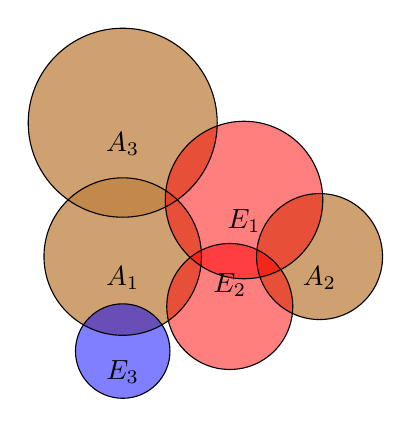
\begin{tikzpicture}

  \def\firstcircle{(25:1.7cm) circle (1cm)}
  \def\secondcircle{(-25:1.5cm) circle (.8cm)}
  \def\thirdcircle{(-90:1.2cm) circle (.6cm)}
  \def\taskcircleA{(0,0) circle(1cm)}
  \def\taskcircleB{(0:2.5cm) circle(.8cm)}
  \def\taskcircleC{(90:1.7cm) circle(1.2cm)}

  \begin{scope}
      \fill[brown,fill opacity=0.75] \taskcircleA;
      \fill[brown,fill opacity=0.75] \taskcircleB;
      \fill[brown,fill opacity=0.75] \taskcircleC;

      \fill[red,fill opacity=0.5] \firstcircle;
      \fill[red,fill opacity=0.5] \secondcircle;
      \fill[blue,fill opacity=0.5] \thirdcircle;

      \draw \taskcircleA node[below] {$A_1$};
      \draw \taskcircleB node[below] {$A_2$};
      \draw \taskcircleC node[below] {$A_3$};

      \draw \firstcircle node[below] {$E_1$};
      \draw \secondcircle node [above] {$E_2$};
      \draw \thirdcircle node [below] {$E_3$};

  \end{scope}

\end{tikzpicture}
\end{document}
